\documentclass[10pt,journal,compsoc]{IEEEtran}
\newif\ifpeerreview

%%% Important: for camera ready submissions, replace the following line
%%% with \peerreviewfalse
\peerreviewfalse


\usepackage[nocompress]{cite}
\usepackage{url}
\usepackage{amsmath,amssymb,graphicx}
\usepackage{multirow}
\usepackage{hyperref}
\usepackage[switch]{lineno}

% Insert your paper ID and information below
\newcommand{\paperID}{XXXX}

% Enter your paper title below
\title{Ensemble-based Defensive Pipeline Against Adversarial Attacks}

% Enter your author information before
% Note this is only necessary for the camera review. Submissions are anonymized.
\author{Junbo Huang (1004280422), Jason Tang (1004221326)}


\begin{document}

\IEEEtitleabstractindextext{%
\begin{abstract}
Adversarial attacks present a significant security risk to most modern usages of machine learning, especially in the field of computer vision. To our knowledge, there are no defense systems that can provide robustness against white-box adversarial attacks with a computationally efficient run time. For the white-box setting, we propose GPEnsemble, a gaussian pyramid inspired ensemble defense system combined with an adversarially trained DnCNN denoiser preprocessor. Our system outperforms previous defense systems (Ensemble Adversarial Training and Fast Adversarial Training) at the strongest tested attack (C\&W), with our system retaining 72.6\% accuracy at the highest tested perturbation level while the other systems falling to 7.4\% and 9.6\% accuracy, respectively.\\

The code for this project is available at: \href{https://github.com/JasonTang99/gaussian-pyramid-defense}{https://github.com/JasonTang99/gaussian-pyramid-defense}
\end{abstract}
}

% Make Title
\maketitle

\section{Introduction} %%%%%%%%%%%%%%%%%%%%%%%%%%%%%%%%%%%
In recent years, machine learning (ML) models have improved dramatically in their ability to perform visual tasks on naturally occurring images. However, most ML systems in use today were designed with minimal consideration of the exploits a malicious actor could employ against these systems. One class of these adversarial attacks focuses specifically on tampering with model integrity such that it outputs incorrect predictions, potentially in a manner benefiting attackers. Some potential exploits include: falsifying cheques, bypassing facial recognition systems, and causing abnormal self-driving car behavior by altering detected road signs. 

These model integrity attacks generally utilize model weights to perform constrained gradient steps in the input image space or to solve constrained optimization problems, both of which generate imperceptibly small perturbations to input images that cause models to produce erroneous outputs. Even in black-box scenarios where attackers have no access to model weights and architecture, there are methods that can learn a substitute clone of the target model and exploit the transferability of adversarial examples to attack black-box models without knowledge of model architecture or even access the same training data \cite{pbba}. This nullifies many attempts of security through obscurity, causing a shift towards defenses in gray-box or white-box scenarios in recent research, where attackers have partial, or even complete access to model architecture, weights, and training data. 

In our project, we propose and analyze the robustness of a novel ensemble-based defense system utilizing different input sizes in the white-box setting. 


\section{Related Work} %%%%%%%%%%%%%%%%%%%%%%%%%%%%%%%%%%%
\subsection{Adversarial Attacks}

Attacks can be generated by solving a constrained optimization problem, which minimizes or bounds a distance metric (e.g. $L_0$, $L_2$, and $L_\infty$) between the clean image and adversarial example. The minimization of image distance encourages imperceptible changes, such that human analysis of adversarial images does not raise concerns.

For standard convolutional neural networks (CNNs), the Fast Gradient Sign Method (FGSM) presents a simple and efficient attack that exploits the existing backpropagation architecture in modern neural networks to efficiently calculate and ascend along the gradient of the loss function with respect to the input image \cite{fgsm}. This gradient step can also be repeated iteratively within the constrained space using Projected Gradient Descent (PGD), and with random nearby initializations to create more powerful attacks \cite{pgd}. Carlini and Wagner (C\&W) present another strong attack which breaks several previously effective defenses by directly optimizing the constrained optimization problem using a margin loss \cite{cw}. Lastly, the Skip Gradient Method (SGM) is a recent technique which exploits skip connections in neural networks with residual connections to pass gradients through the model more directly \cite{sgm}.

\subsection{Ensemble Defenses}
To address this, many defenses have been proposed and defeated in an ongoing arms race within this field. A popular defense is to smooth out the model gradients to near 0 such that the adversarial gradient steps are no longer useful \cite{lbfgs} \cite{dd}. However, these gradient masking techniques only obfuscate the gradient information, they do not remove the existence of adversarial images. Attackers can effectively bypass this defense by learning a substitute model with useful gradients which can exploit the transferability of adversarial examples to attack the masked target model \cite{pbba}. Another common defense relies on numerically unstable or non-differentiable functions such as sigmoids, median filters, and step functions. However, attackers can simply replace these problematic layers with a differentiable approximation, and optimize along the slightly incorrect gradients to create adversarial examples \cite{bpda}. 

As such, some researchers have begun using ensemble-based methods with the goal of improving model robustness to adversarial examples through diverse ensemble members. One method uses a regularizer term encouraging orthogonality in non-maximal predictions between ensemble members \cite{diversity}, and another uses different numerical precisions between members \cite{empir}. However, both of these methods were broken by running PGD until convergence and by approximating the numerically unstable majority vote with an average, respectively \cite{survey}. A successful black-box defense is Ensemble Adversarial Training, which utilizes adversarial examples generated using R+FGSM (a FGSM variation with a random step) on other ensemble members to perform adversarial training \cite{eat}. This corresponds to the method attackers used to attack vanilla adversarial training \cite{pbba}, which likely leads to the superior robustness seen with this defense. This idea was extended to the white-box setting with appropriate attack parameter tuning in Fast Adversarial Training \cite{fat}.


\begin{figure}[!t]
\centering
    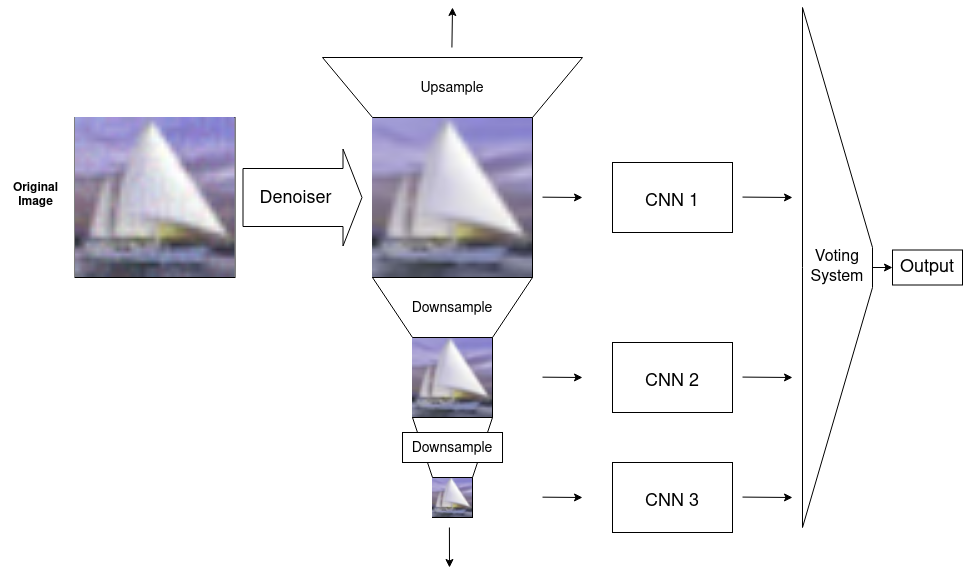
\includegraphics[scale=0.25]{images/diagram.png}
    \caption{Illustration of our proposed method.}
    \label{fig:diagram}
\end{figure}

\subsection{Denoising Defenses}
Many different denoising techniques have been proposed as a defensive mechanism against adversarial attacks. Traditional denoising methods such as Gaussian, Bilateral, Non-local Means, and Total Variation have all proven useful in removing noise in adversarially perturbed images. Simply applying defensive denoising with TV and NLM can remove major parts of the universal adversarial perturbations in images and improve classification performance \cite{cite11}. A more recent feature denoising \cite{cite12} method  was designed to incorporate NLM as intermediate blocks in the convolutional network of the classifiers; these denoising blocks can be trained to directly remove noises caused by adversarial perturbations on intermediate features.

Deep learning based architectures are also very effective as denoising preprocessors. Convolutional neural networks such as Denoising Autoencoders (DAE) and U-Net have a great capacity for learning and removing adversarial noise. The deep denoising sparse autoencoder (DDSA) \cite{cite13} method intends to learn a representation extracted from the autoencoder that is robust to adversarial perturbations by adding a sparsity constraint in the bottleneck phase to enforce the extraction of only meaningful and relevant features. However, such bottleneck structures between the encoder and the decoder might hinder the transmission of fine details necessary for high-resolution image reconstruction. A denoising U-net (DUNET) \cite{cite14} addresses this problem by adding lateral connections and incorporating residual learning. DUNET learns the adversarial noise with a loss function guided by a high-level representation of the images. The DnCNN \cite{cite15} architecture has also seen lots of success in its capability and efficiency in image denoising. It is a feed-forward neural network that leverages batch normalization and residual learning techniques to estimate the residual in the image, which suggests that it could also potentially be an effective denoising preprocessor.

% I'm not sure why but putting it here works
\begin{figure*}[!h]
\centering
    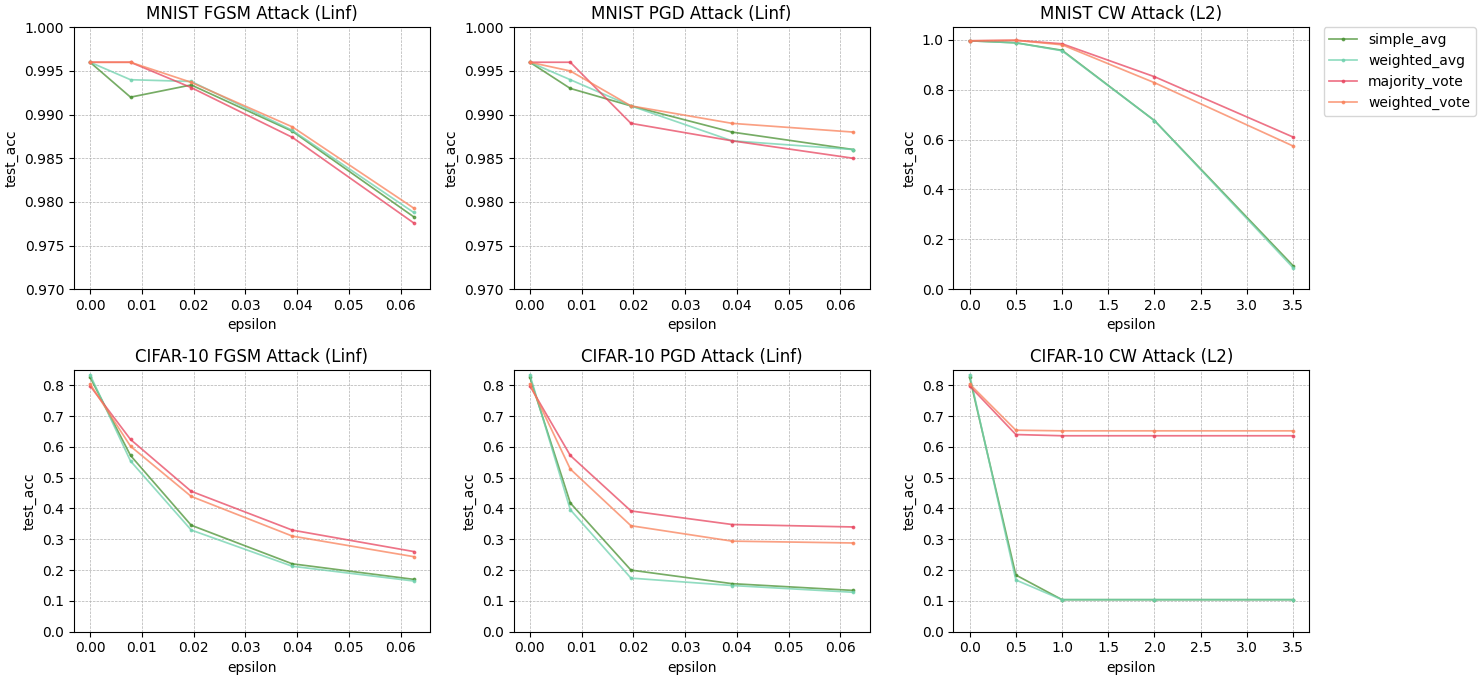
\includegraphics[width=1.8\columnwidth]{images/voting_methods.png}
    \caption{Comparison of different voting methods. (Ensemble only)}
    \label{fig:voting}
\end{figure*}

\section{Proposed Method} %%%%%%%%%%%%%%%%%%%%%%%%%%%%%%%%%%%
\subsection{Gaussian Pyramid Ensemble}
We introduce GPEnsemble, a gaussian pyramid inspired ensemble-based defense system for image classification. Each ensemble member receives a different resized version of the input image (see Fig. \ref{fig:diagram}), where the resampling is done using the same multiplicative scaling factor in each direction for simplicity. We explored using different input scaling factors $[2.0, 1.1]$, as smaller scales allow for more ensemble members with better space efficiency.

The motivation behind this ensemble construction is that the attacker will need to essentially trick each ensemble member at the same time, where each member is diverse and difficult to simultaneously fool due to the varied input sizes. Additionally, downsampling destroys image information so attacks may need to attack entire patches of the input image to target a downsampled model. However, this also produces a drop in accuracy, which is why we also include upsampled input images to alleviate this performance loss.  

Each input is then passed through a vanilla Resnet \cite{resnet} model (18-layer), which is pre-trained on ImageNet and then finetuned on the associated input size. The resulting outputs are then combined in the following ways:
\begin{itemize}[leftmargin=*]
\item \textit{Uniform Average Outputs:} A linear baseline averaging all outputs uniformly.
\item \textit{Weighted Average Outputs:} Performance scaled weights will likely improve performance on clean inputs, but could lead to targeted attacks on the highest performing models.
\item \textit{Uniform Majority Vote} (non-differentiable): Equal votes introduces a non-differentiable step.
\item \textit{Weighted Majority Vote} (non-differentiable): Better accuracy on clean inputs, but may be more vulnerable.
\end{itemize}

We choose not to consider any random selection methods where a single ensemble model is selected to make the classification decision as it allows attackers to target a single ensemble member and to simply repeatedly submit the adversarial attack until the targeted member is inevitably randomly selected. 


\subsection{Denoising Preprocessor}
Before passing the input images through the ensemble model, a DnCNN-based denoiser is applied as a preprocessor in the first stage of our defensive pipeline. The DnCNN denoiser was trained with adversarial examples generated by different attack methods on a range of perturbation levels, which should remove major parts of the adversarial perturbations and restore the original structures in the input images. As seen in recent literature, deep denoisers can be quite effective as a defensive measure. We adopted the stock 17-layer DnCNN architecture and cut it down to a 7-layer model to save training time. The biases in the model are also disabled as we think it would provide better generalization, especially on unseen noises.



\section{Evaluation} %%%%%%%%%%%%%%%%%%%%%%%%%%%%%%%%%%%
We examine the robustness of our proposed model with FGSM and PGD attacks on the $L_\infty$ norm, and with C\&W attacks on the $L_2$ norm. Recent literature generally considers $L_\infty$ limits of $[2, 5, 10, 16]$ pixel value changes in FGSM and PGD attacks. Since there is little guidance on similar $L_2$ limits, we calculated the $L_2$ norm of the maximal change in the associated $L_\infty$ limit on a $(3, 32, 32)$ sized CIFAR-10 image to produce the $L_2$ limits of $[0.5, 1.0, 2.0, 3.5]$ for C\&W attacks. 

Additionally, since C\&W doesn’t allow the specification of a $L_2$ limit, we instead run the attack with default parameters and measure the $L_2$ norm of the perturbations. We only count an attack as successful if the perturbation is within the $L_2$ limit and the model prediction changes. 

Since voting methods have no definable gradient, we generate adversarial examples on the associated differentiable substitute and transfer attacks to the target model.

We evaluate our proposed system on both MNIST and CIFAR10 datasets, and compare against both Ensemble Adversarial Training (black-box) and Fast Adversarial (white-box) methods, which we will refer to as EnsAdv and FastAdv, respectively, on CIFAR10.

% DENOISERCOMP
\begin{figure*}[!h]
\centering
    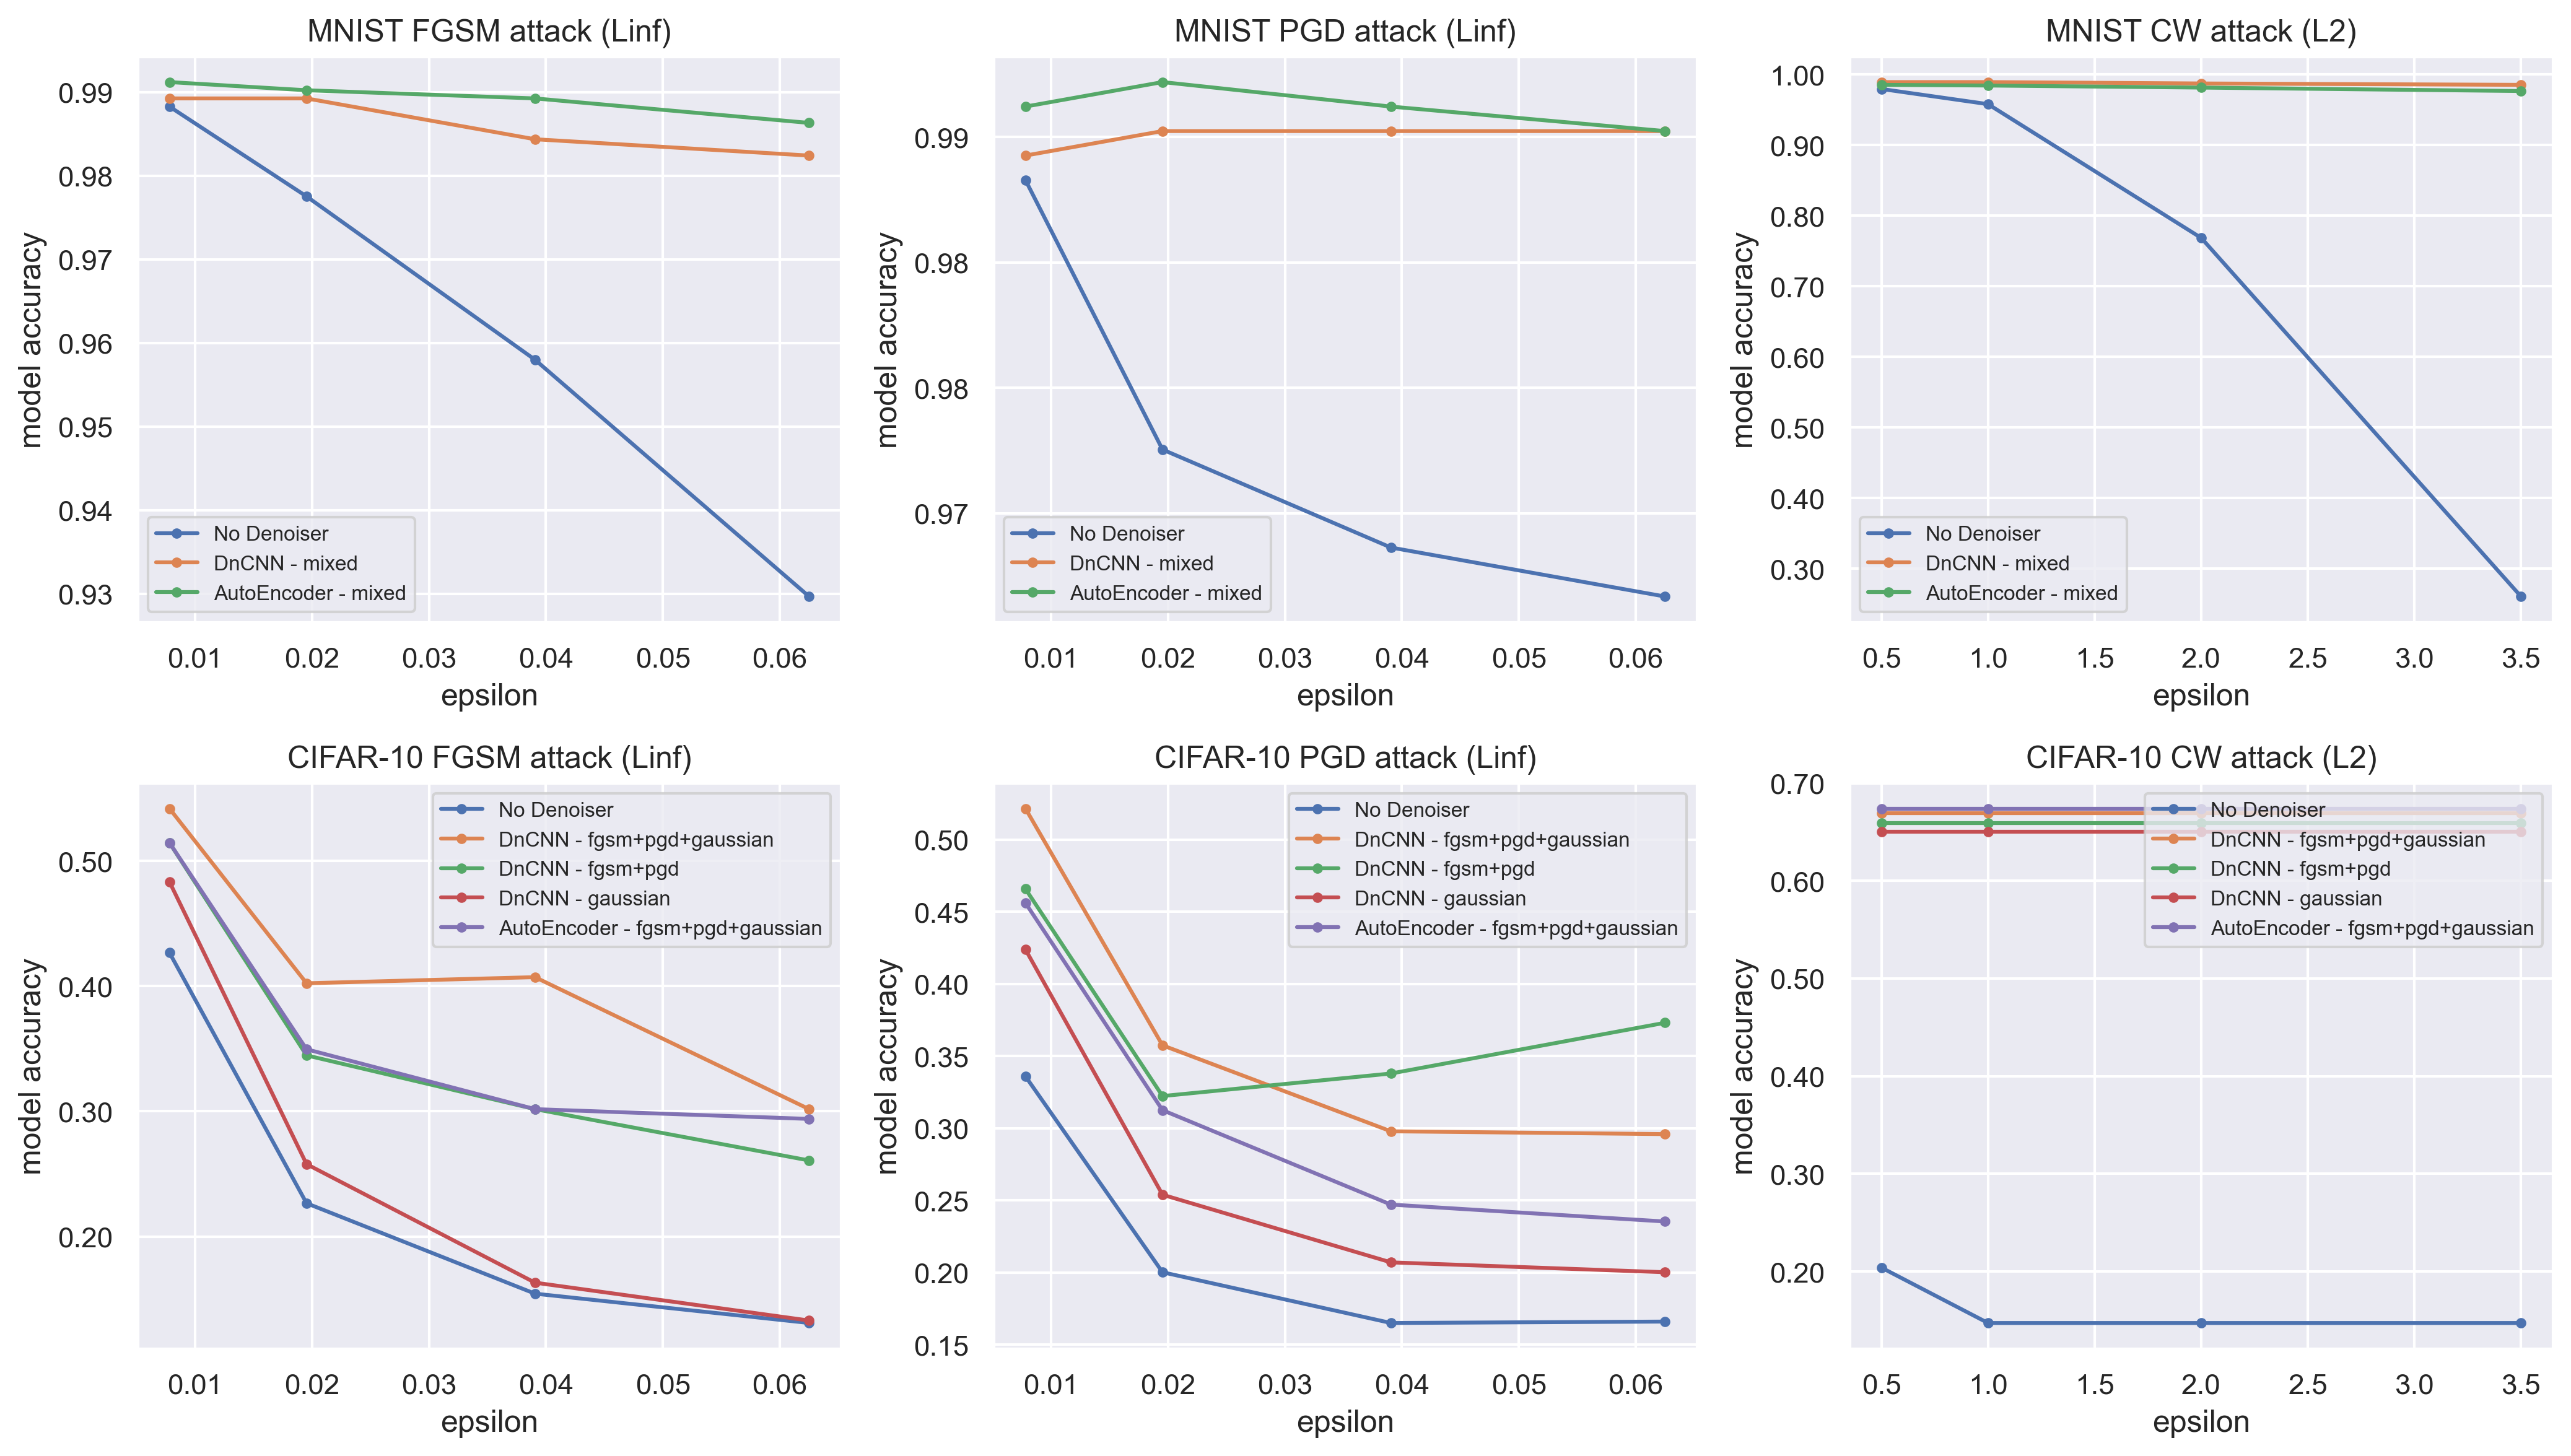
\includegraphics[width=1.8\columnwidth]{images/denoiser_only_result.png}
    \caption{Comparison of denoisers trained with different dataset/architecture (denoiser only)}
    \label{fig:denoisercomp}
\end{figure*}

\section{Results}
\subsection{Ensemble}
In Fig \ref{fig:voting} we analyze the performance of only the ensemble portion (no denoiser) using the different voting methods. We note that our non-differentiable voting methods (majority\_vote, weighted\_vote) generally outperform their differentiable counterparts, especially in the iterative PGD and C\&W attacks. This is likely due to the fact that the more powerful iterative attacks often demonstrate less transferability than one-step attacks \cite{eat}.


% UP_DOWN
\begin{table}[!h]
\renewcommand{\arraystretch}{1.3}
\caption{Comparison of different numbers up samplers and down samplers with a scaling factor of 2 on the FGSM attack. Test accuracies averaged over all epsilons. (Ensemble only)}
\label{table:updown}
\centering
\begin{tabular}{|c|c|c|c|}
\hline
dataset &  up\_samplers &  down\_samplers &  test\_acc \\
 \hline\hline
\multirow{10}{*}{mnist}
   &          0.0 &            0.0 &    96.94\% \\
   &          0.0 &            1.0 &    97.13\% \\
   &          0.0 &            2.0 &    97.65\% \\
   &          0.0 &            3.0 &    96.41\% \\
   &          1.0 &            0.0 &    97.90\% \\
   &          2.0 &            0.0 &    98.82\% \\
   &          3.0 &            0.0 &    \textbf{99.15\%} \\
 \cline{2-4}
   &          1.0 &            1.0 &    98.36\% \\
   &          2.0 &            2.0 &    98.88\% \\
   &          3.0 &            3.0 &    \textbf{99.01\%} \\
\hline\hline
\multirow{10}{*}{cifar10}
 &          0.0 &            0.0 &    33.21\% \\
 &          0.0 &            1.0 &    36.43\% \\
 &          0.0 &            2.0 &    39.91\% \\
 &          0.0 &            3.0 &    \textbf{40.95\%} \\
 &          1.0 &            0.0 &    37.37\% \\
 &          2.0 &            0.0 &    39.93\% \\
 &          3.0 &            0.0 &    \textbf{40.34\%} \\
  \cline{2-4}
 &          1.0 &            1.0 &    40.36\% \\
 &          2.0 &            2.0 &    44.54\% \\
 &          3.0 &            3.0 &    \textbf{45.48\%} \\
\hline
\end{tabular}
\end{table}

In Table \ref{table:updown}, we see that upsamplers are generally more advantageous to have compared to downsamplers. However, due to the exponential space increase required to use these upsamplers, we also utilize downsamplers to increase the ensemble size and robustness. 

% SCALE
\begin{table}[!h]
\renewcommand{\arraystretch}{1.3}
\caption{Comparing scaling factors of 2.0 and 1.1. Test accuracy averaged over epsilons. (Ensemble only)}
\label{table:scale}
\centering
\begin{tabular}{|c|c|c|c|}
\hline
dataset & attack &  scaling, up, down &  test\_acc \\
\hline\hline
\multirow{12}{*}{mnist} 
   &        \multirow{4}{*}{fgsm} &             1.1, 3, 3 &   98.44\% \\
   &         &             1.1, 5, 5 &   98.65\% \\
   &         &             1.1, 7, 7 &   98.79\% \\
   &         &             2.0, 3, 3 &   \textbf{99.01\%} \\
   \cline{2-4}
 &         \multirow{4}{*}{pgd} &             1.1, 3, 3 &   98.65\% \\
   &          &             1.1, 5, 5 &   98.70\% \\
   &          &             1.1, 7, 7 &   98.62\% \\
   &          &             2.0, 3, 3 &   \textbf{99.10\%} \\
   \cline{2-4}
&          \multirow{4}{*}{cw} &             1.1, 3, 3 &   67.20\% \\
   &           &             1.1, 5, 5 &   75.99\% \\
   &           &             1.1, 7, 7 &   77.09\% \\
   &           &             2.0, 3, 3 &   \textbf{81.15\%} \\
 \hline\hline
\multirow{12}{*}{cifar10} 
 & \multirow{4}{*}{fgsm} &             1.1, 3, 3 &   43.25\% \\
 &         &             1.1, 5, 5 &   43.93\% \\
 &         &             1.1, 7, 7 &   \textbf{45.25\%} \\
 &         &             2.0, 3, 3 &   \textbf{45.48\%} \\
 \cline{2-4}
 & \multirow{4}{*}{pgd} &             1.1, 3, 3 &   47.78\% \\
 &          &             1.1, 5, 5 &   49.89\% \\
 &          &             1.1, 7, 7 &   \textbf{51.86\%} \\
 &          &             2.0, 3, 3 &   40.62\% \\
 \cline{2-4}
 & \multirow{4}{*}{cw} &             1.1, 3, 3 &   37.91\% \\
 &           &             1.1, 5, 5 &   45.95\% \\
 &           &             1.1, 7, 7 &   \textbf{47.17\%} \\
 &           &             2.0, 3, 3 &   \textbf{46.98\%} \\
   \hline
\end{tabular}\end{table}


\begin{figure}[!h]
\centering
    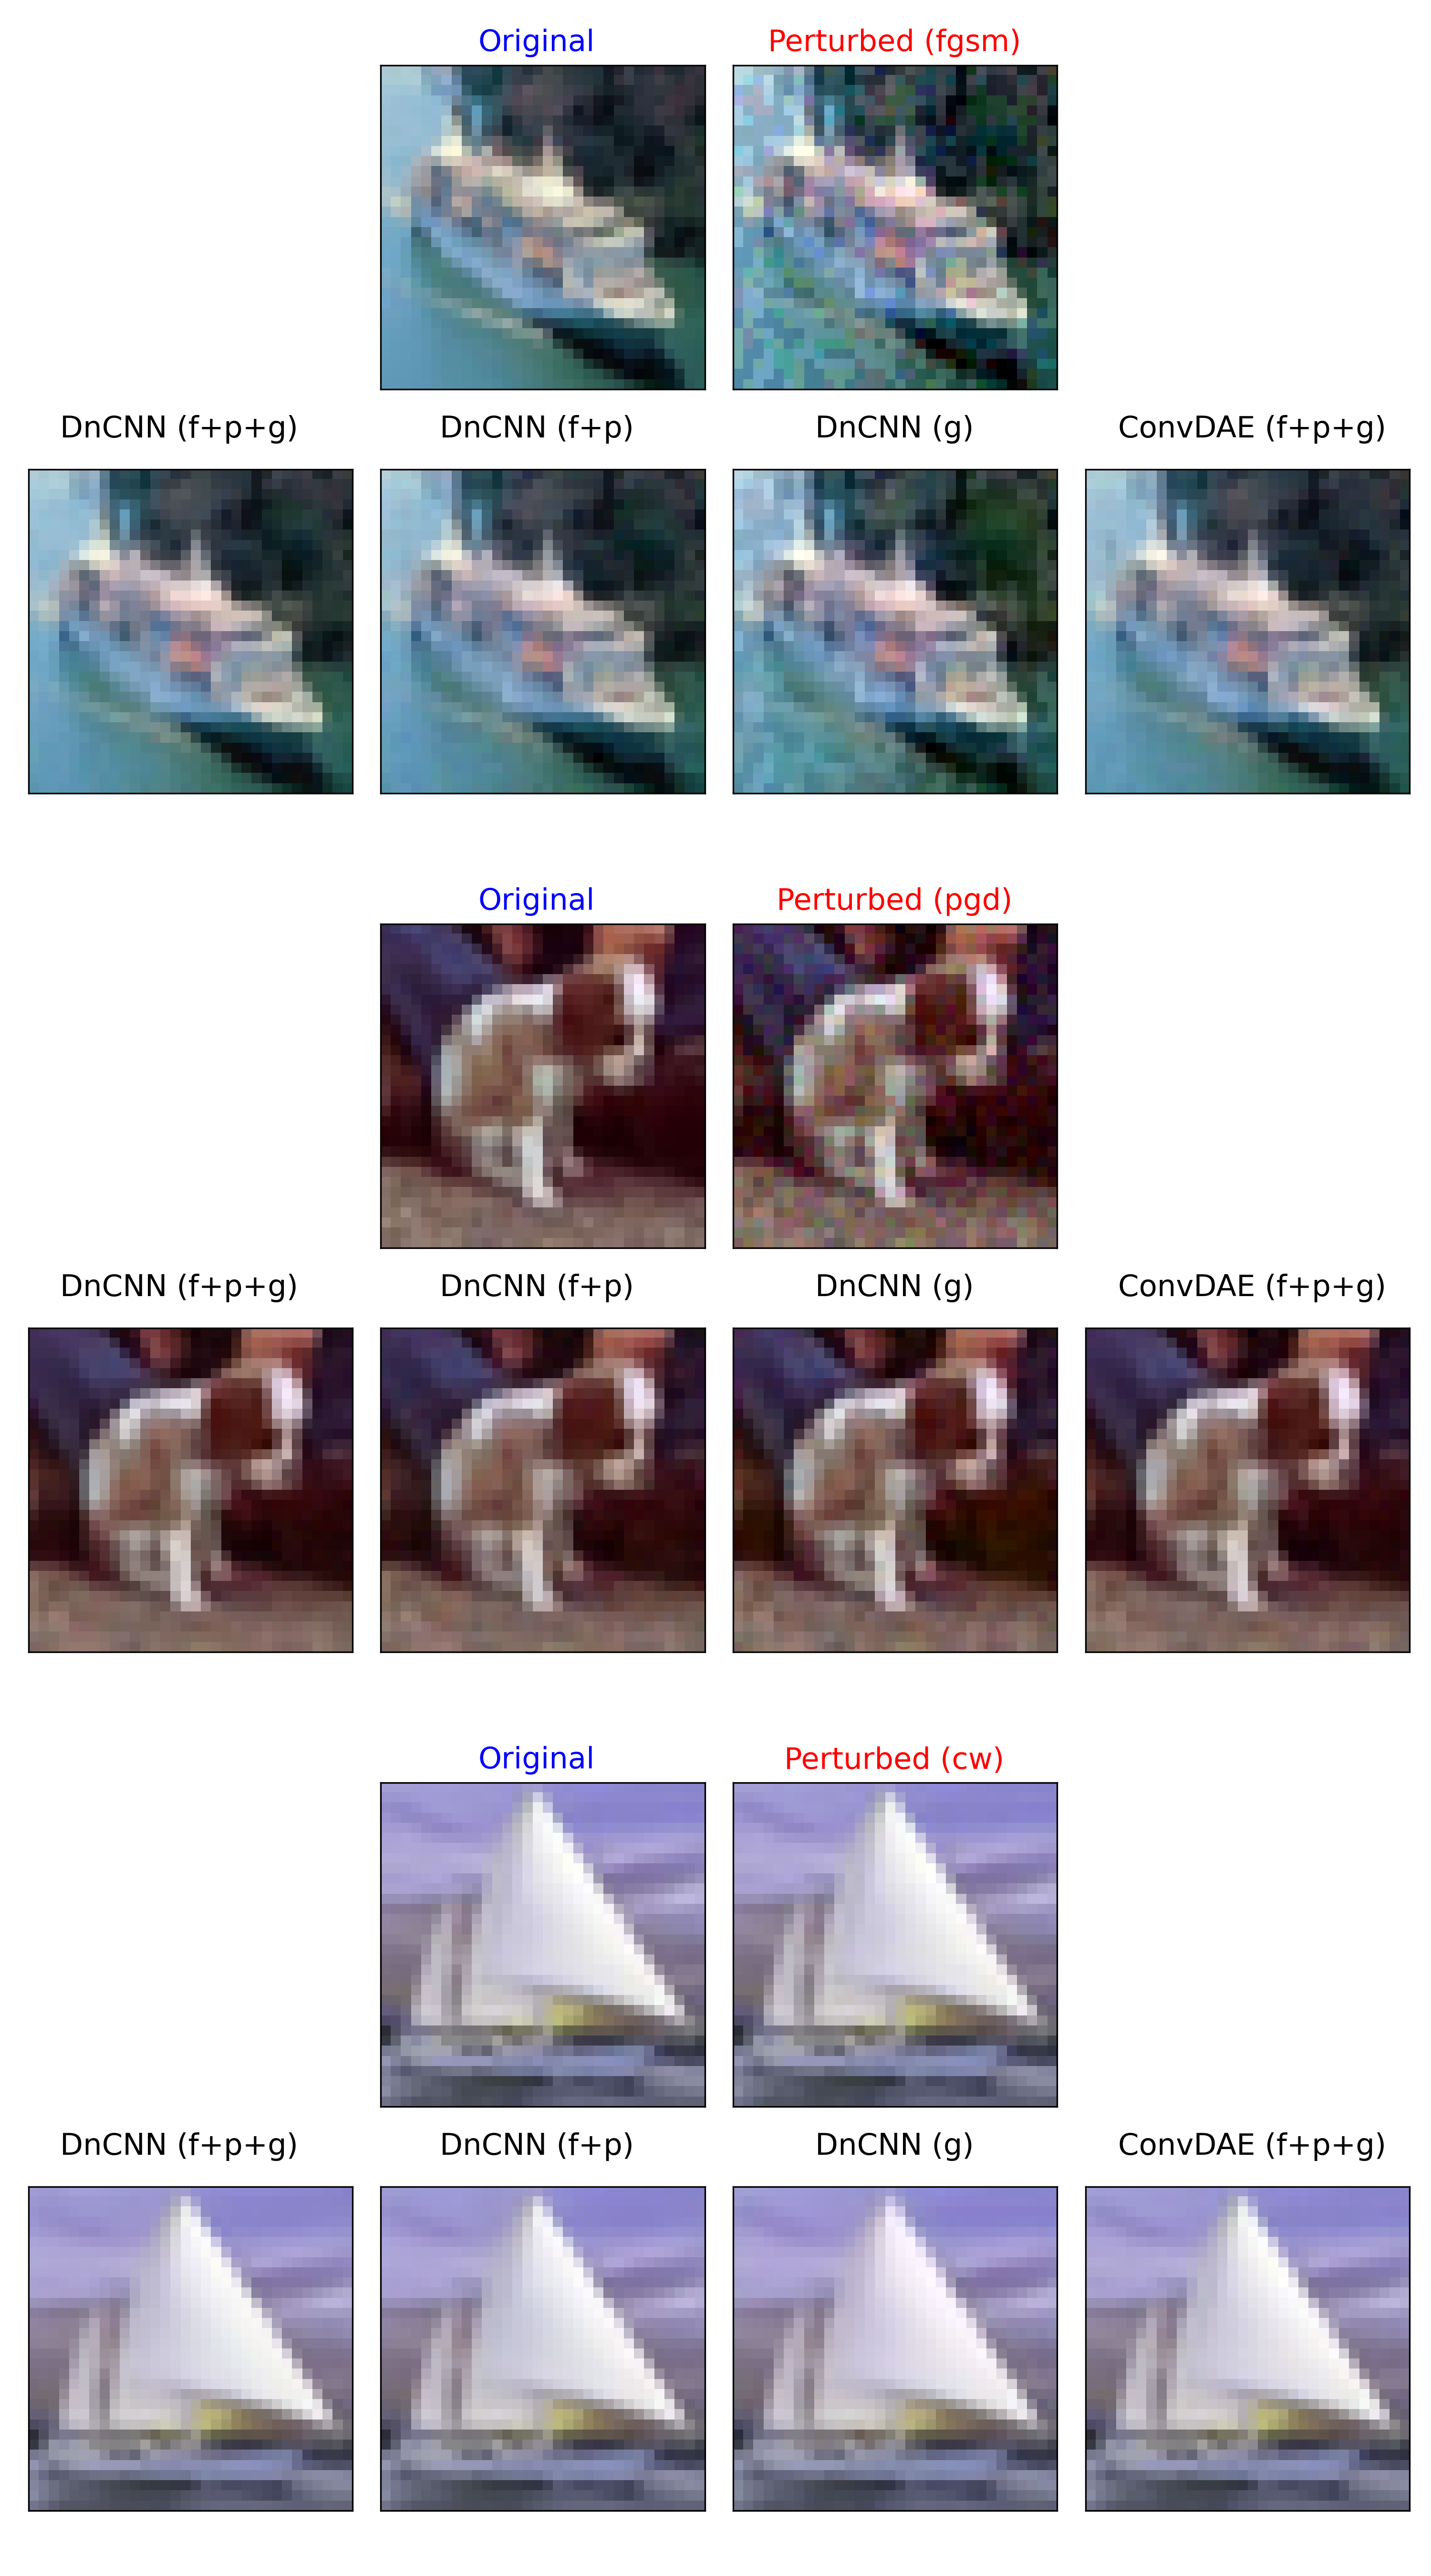
\includegraphics[width=0.9\columnwidth]{images/denoiser_sample.png}
    \caption{Sample adversarial images and denoised outputs}
    \label{fig:advsample}
\end{figure}

We also considered lowering the scale factor from 2.0 to 1.1, with results in Table \ref{table:scale}. The lower scaling factor allows the addition of more upsamplers and downsamplers before running into memory space constraints or complete loss of image information. The results show that using a factor of 2.0 will always dominate a factor of 1.1 when both have the same ensemble member counts, but using the ability to have more ensemble members in 1.1 produces better results in the more challenging CIFAR10 dataset.

\subsection{Denoising}
For evaluating the denoising performance, we were primarily focusing on the CIFAR10 dataset as it is more representative in real-world scenarios. Our custom training dataset contains adversarial examples generated by FGSM and PGD methods on a range of $l_{\infty}$ norms, and additional noisy examples with added Gaussian noise. It is worth noting that we did not include C\&W examples, as images perturbed by the C\&W attack have no perceivable noise and are structurally similar to the original images (See Table \ref{table:psnr} and Fig. \ref{fig:advsample}). Therefore, training the denoisers on these examples will give us no benefit in learning and image reconstruction performance. 

We conducted ablation studies by comparing denoiser models trained on different combinations of training examples and evaluated their respective PSNR, SSIM value in image restoration, and classification accuracy in each attack scenario. We have discovered that training with gaussian noise examples generally leads to improved denoising and generalization performance. As an additional comparative analysis, we have compared the denoising performance of our DnCNN model with a 10-layer convolutional autoencoder (ConvDAE) \cite{rednet} trained on the same dataset.

In Table \ref{table:psnr} and \ref{table:acc}, we see that the DnCNN denoiser trained with FGSM, PGD, and gaussian noise examples had the best overall performance under FGSM and PGD attacks, averaging a 17.9\% and 15.2\% accuracy increase compared to the baseline model without a denoiser. We also observed that the effect of C\&W attack was alleviated almost completely with all 4 denoisers, suggesting that image smoothing can be the major factor in reverting the perturbations in C\&W attacked images. In Fig. \ref{fig:advsample}, we can visually observe that denoisers trained with mixed training examples yielded the best overall image reconstruction quality. Overall, the DnCNN model achieved better defensive denoising performance compared to the ConvDAE model on the CIFAR10 dataset, while being more lightweight and easy to train.


% denoiser results and figures
\begin{table}[!h]
\renewcommand{\arraystretch}{1.3}
\caption{Average PSNR and SSIM values of restored images in FGSM ($l_{\infty}$, eps=0.0625), PGD ($l_{\infty}$, eps=0.0625), and C\&W attacks ($l_{2}$, eps=3.5) on CIFAR-10}
\label{table:psnr}
\centering
\begin{tabular}{|l | c||c|c |}
\hline
Attack & Denoiser & PSNR (dB) & SSIM \\
\hline\hline
\multirow{5}{*}{FGSM}
& DnCNN - (fgsm+pgd+gaussian) & \textbf{31.816} & \textbf{0.974}\\
\cline{2-4}
& DnCNN - (fgsm+pgd) &30.648 & 0.965\\
\cline{2-4}
& DnCNN - (gaussian) &25.857 & 0.888\\
\cline{2-4}
& ConvDAE - (fgsm+pgd+gaussian) &28.883 & 0.948\\
\cline{2-4}
& Baseline (No Denoiser) &24.207 & 0.843\\
\hline \hline
% \hline
% & Denoisers & PSNR (dB) & SSIM \\
% \hline
\multirow{5}{*}{PGD}
& DnCNN - (fgsm+pgd+gaussian) & \textbf{33.626} & \textbf{0.979}\\
\cline{2-4}
& DnCNN - (fgsm+pgd) &32.072 & 0.971\\
\cline{2-4}
& DnCNN - (gaussian) &32.074 & 0.970\\
\cline{2-4}
& ConvDAE - (fgsm+pgd+gaussian) &33.398 & 0.979\\
\cline{2-4}
& Baseline (No Denoiser) &28.730 & 0.931\\
\hline\hline
\multirow{5}{*}{C\&W}
% Denoisers & PSNR (dB) & SSIM \\
& DnCNN - (fgsm+pgd+gaussian) & 39.656 & 0.994\\
\cline{2-4}
& DnCNN - (fgsm+pgd) &39.764 & 0.994\\
\cline{2-4}
& DnCNN - (gaussian) &36.873 & 0.987\\
\cline{2-4}
& ConvDAE - (fgsm+pgd+gaussian) &\textbf{44.432} & \textbf{0.998}\\
\cline{2-4}
& Baseline (No Denoiser) &$\infty$ & 0.999\\
\hline

\end{tabular}
\end{table}

\begin{table}[!h]
\renewcommand{\arraystretch}{1.3}
\caption{CIFAR-10 classification accuracy averaged over epsilons (denoisers only)}
\label{table:acc}
\centering
\begin{tabular}{|l||c|c|c|}
\hline
\multirow{2}{*}{Denoiser}
 & \multicolumn{3}{|c|}{Test Accuracy} \\
 \cline{2-4}
 & FGSM & PGD & C\&W \\
\hline\hline
DnCNN - (fgsm+pgd+gaussian) & \textbf{41.33\%} & \textbf{36.82\%} & 66.89\%\\
\hline
DnCNN - (fgsm+pgd) &35.55\% & 37.48\% & 65.92\%\\
\hline
DnCNN - (gaussian) &25.93\% & 27.12\% & 65.04\%\\
\hline
ConvDAE - (fgsm+pgd+gaussian) &36.5\% & 31.27\% & \textbf{67.38\%}\\
\hline
Baseline (No Denoiser) &23.46\% & 21.68\% & 16.16\%\\
\hline
\end{tabular}
\end{table}





% \begin{figure}[!h]
% \centering
%     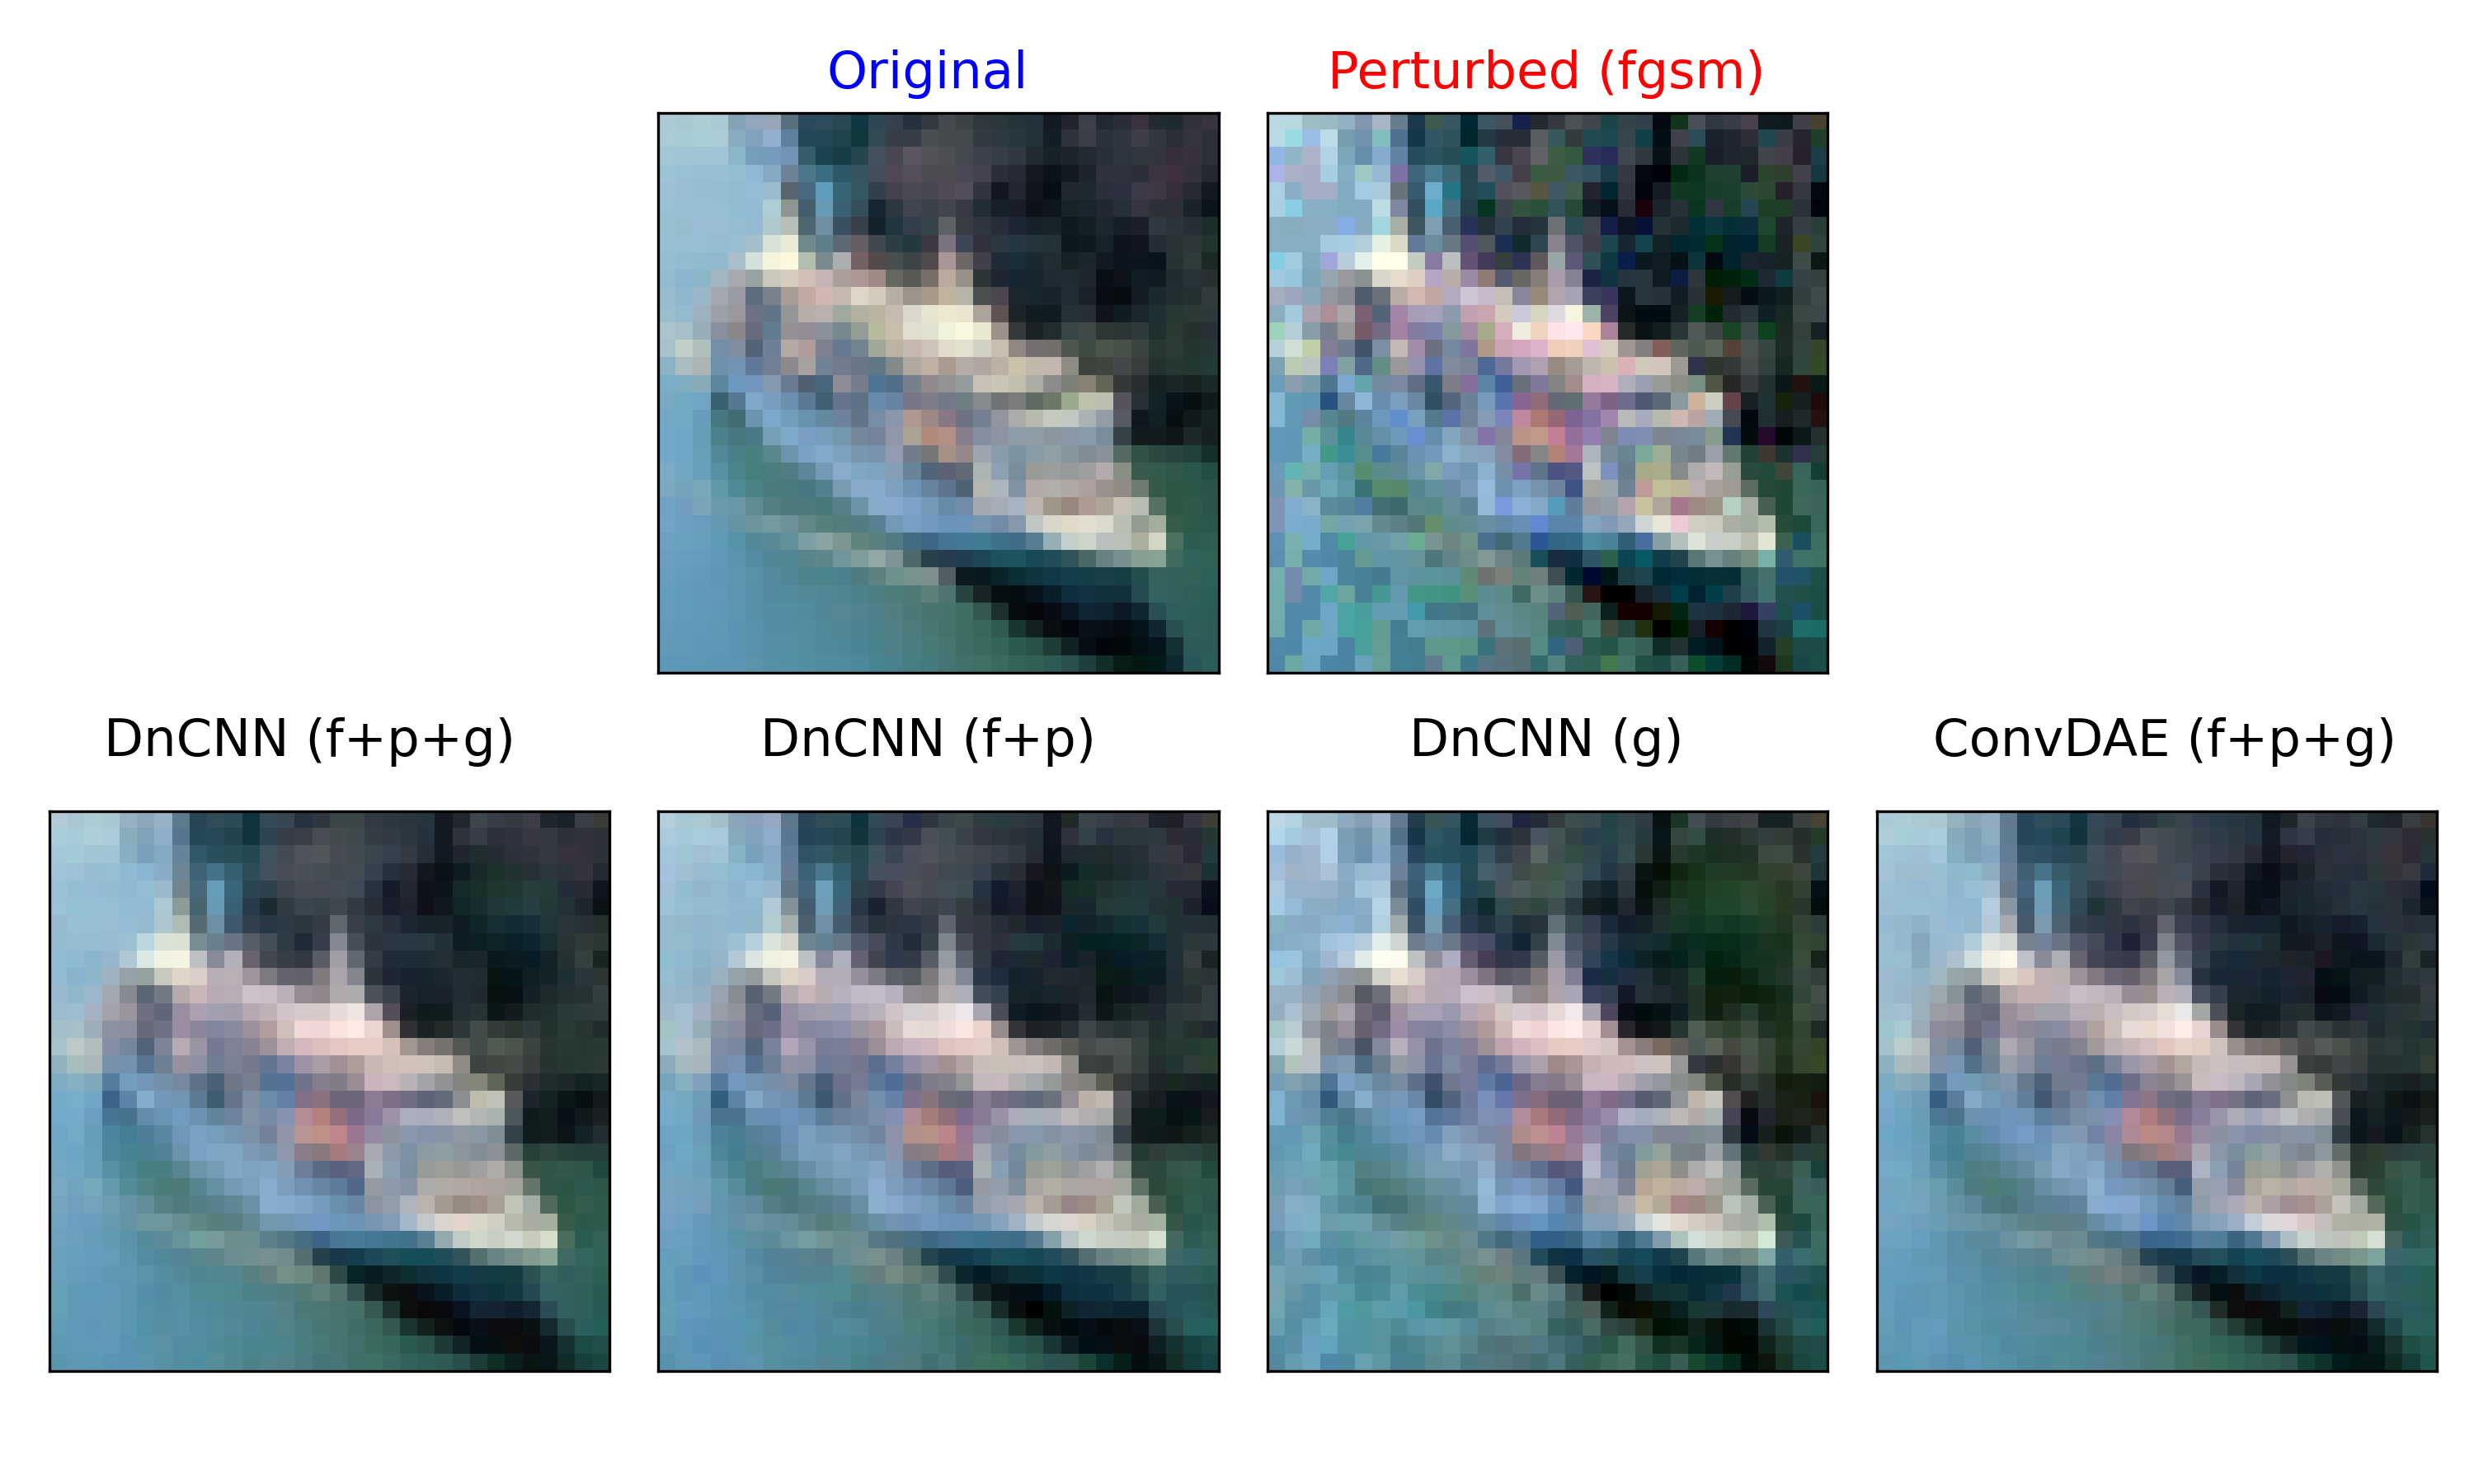
\includegraphics[width=\columnwidth]{images/fgsm_denoiser_comp2.png}
%     \caption{Sample FGSM image and denoiser outputs}
%     \label{fig:fgsm}
% \end{figure}

% \begin{figure}[!h]
% \centering
%     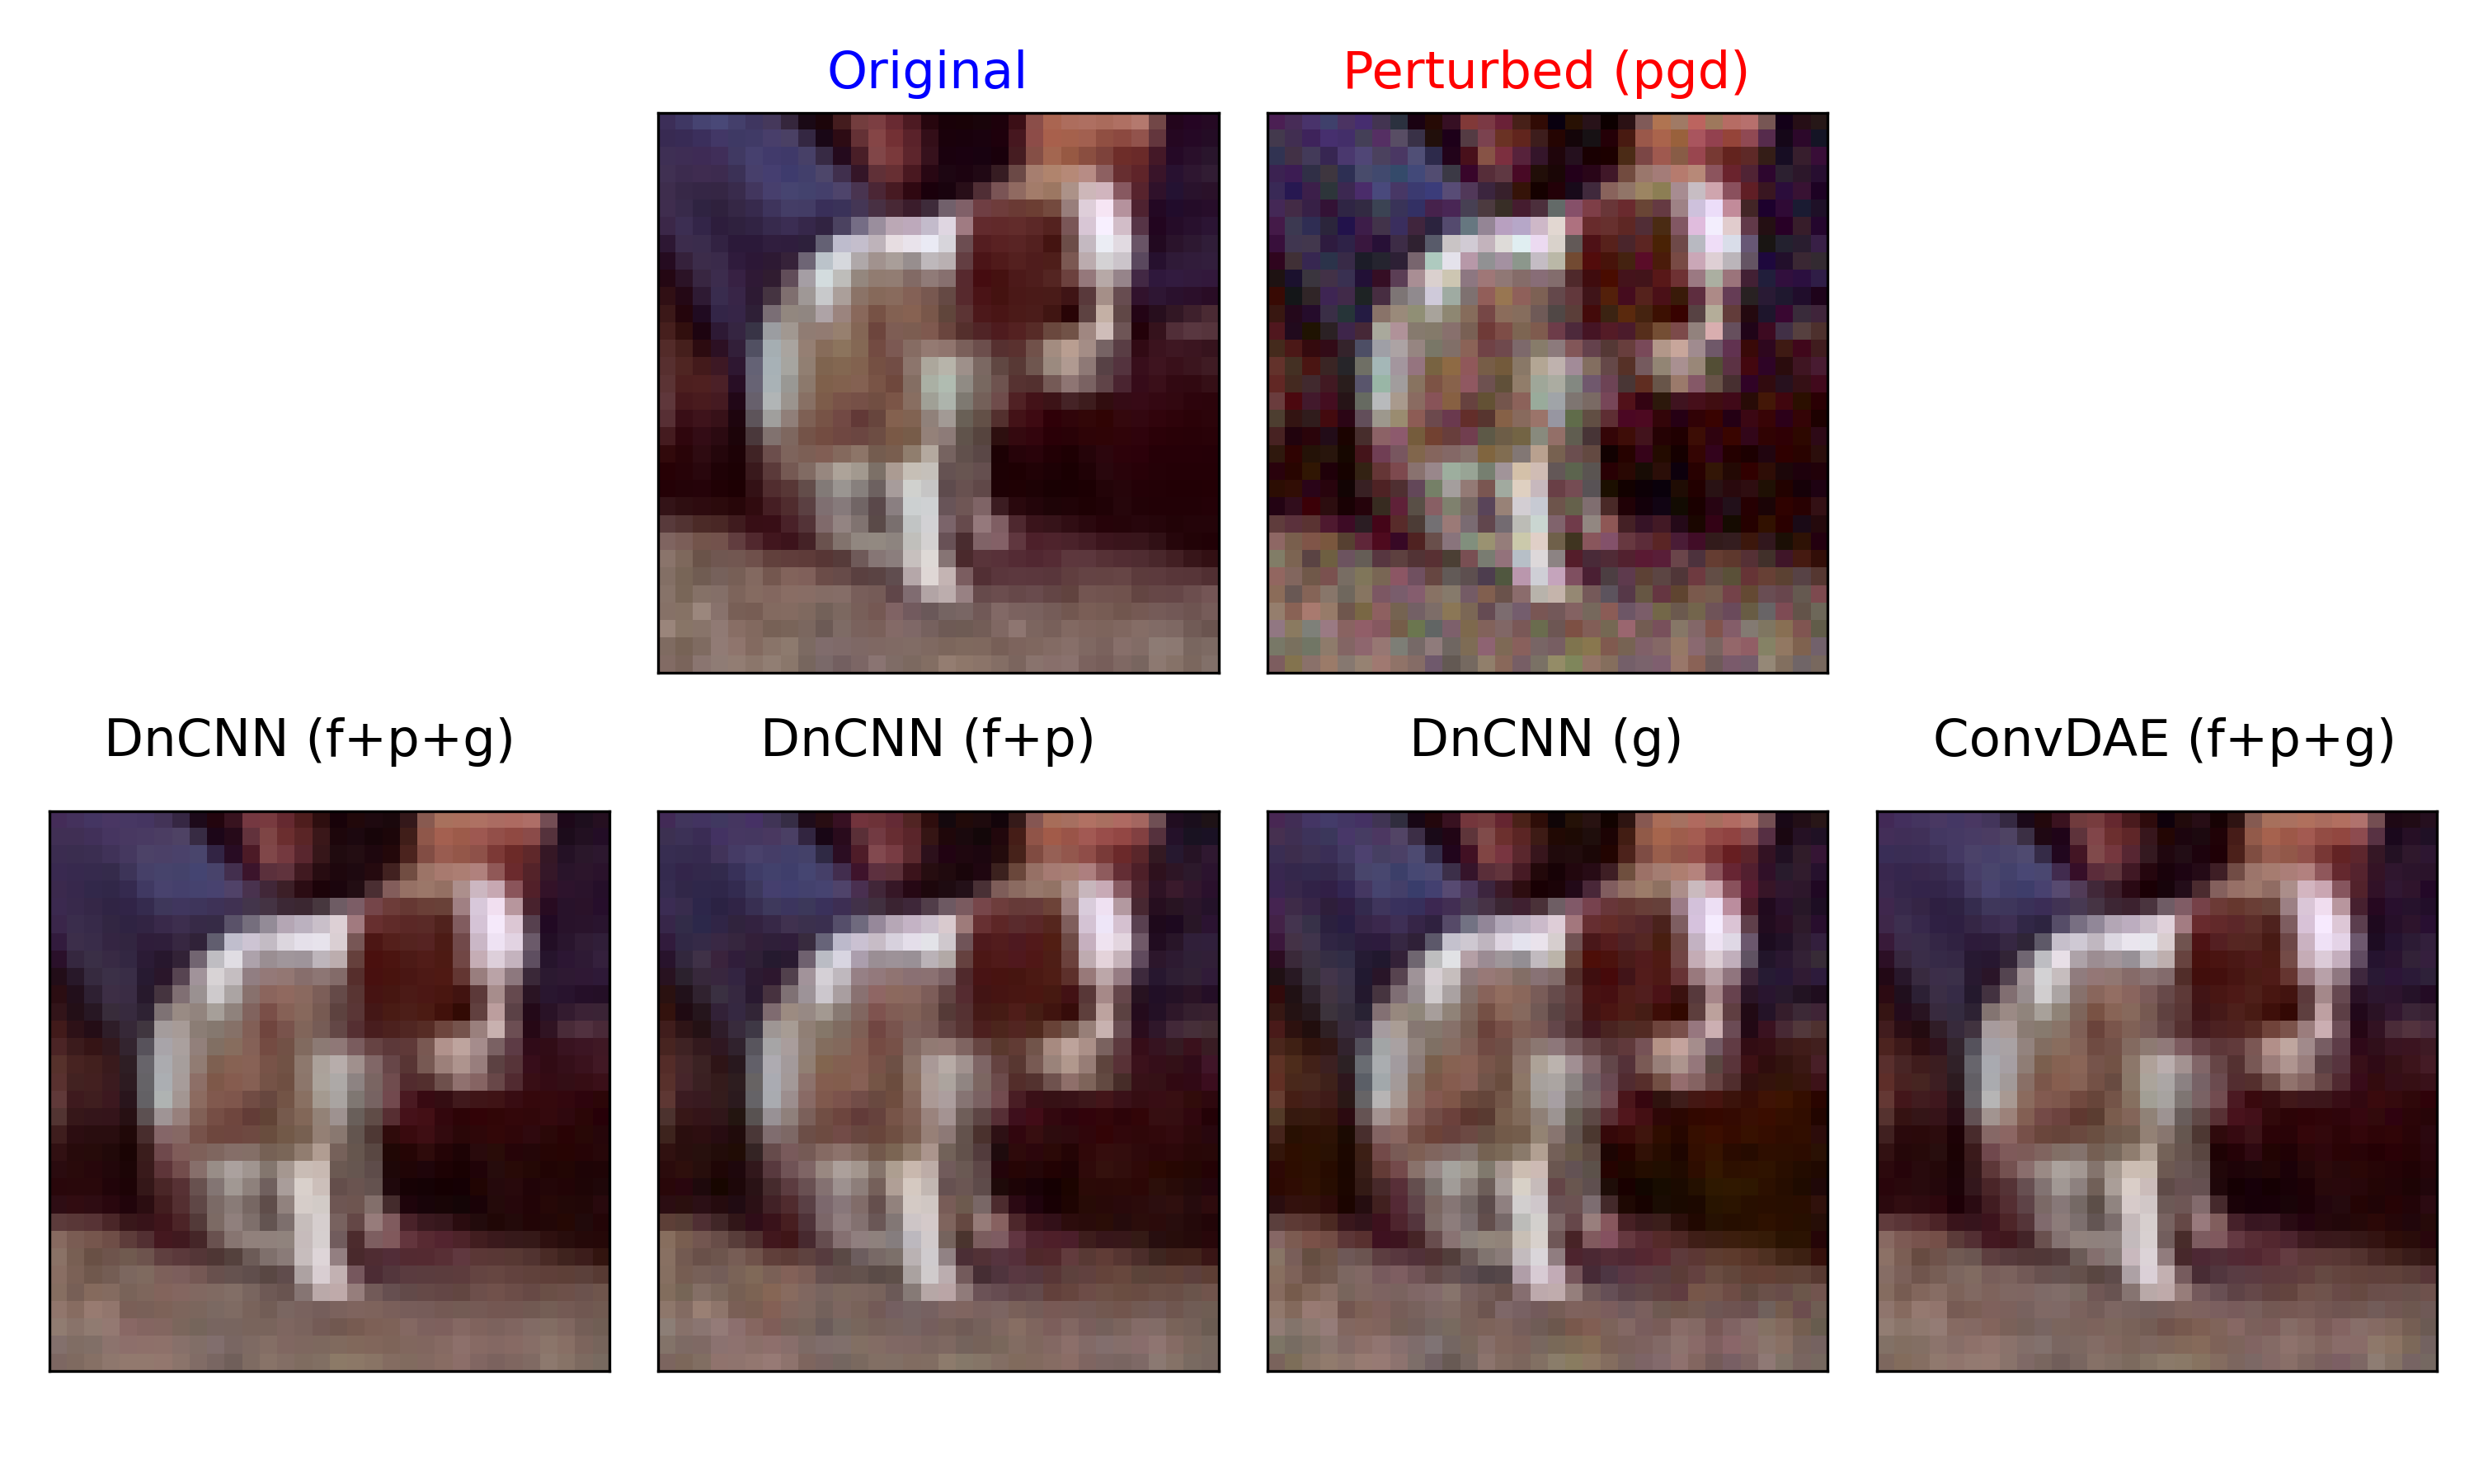
\includegraphics[width=\columnwidth]{images/pgd_denoiser_comp2.png}
%     \caption{Sample PGD image and denoiser outputs}
%     \label{fig:pgd}
% \end{figure}

% \begin{figure}[!h]
% \centering
%     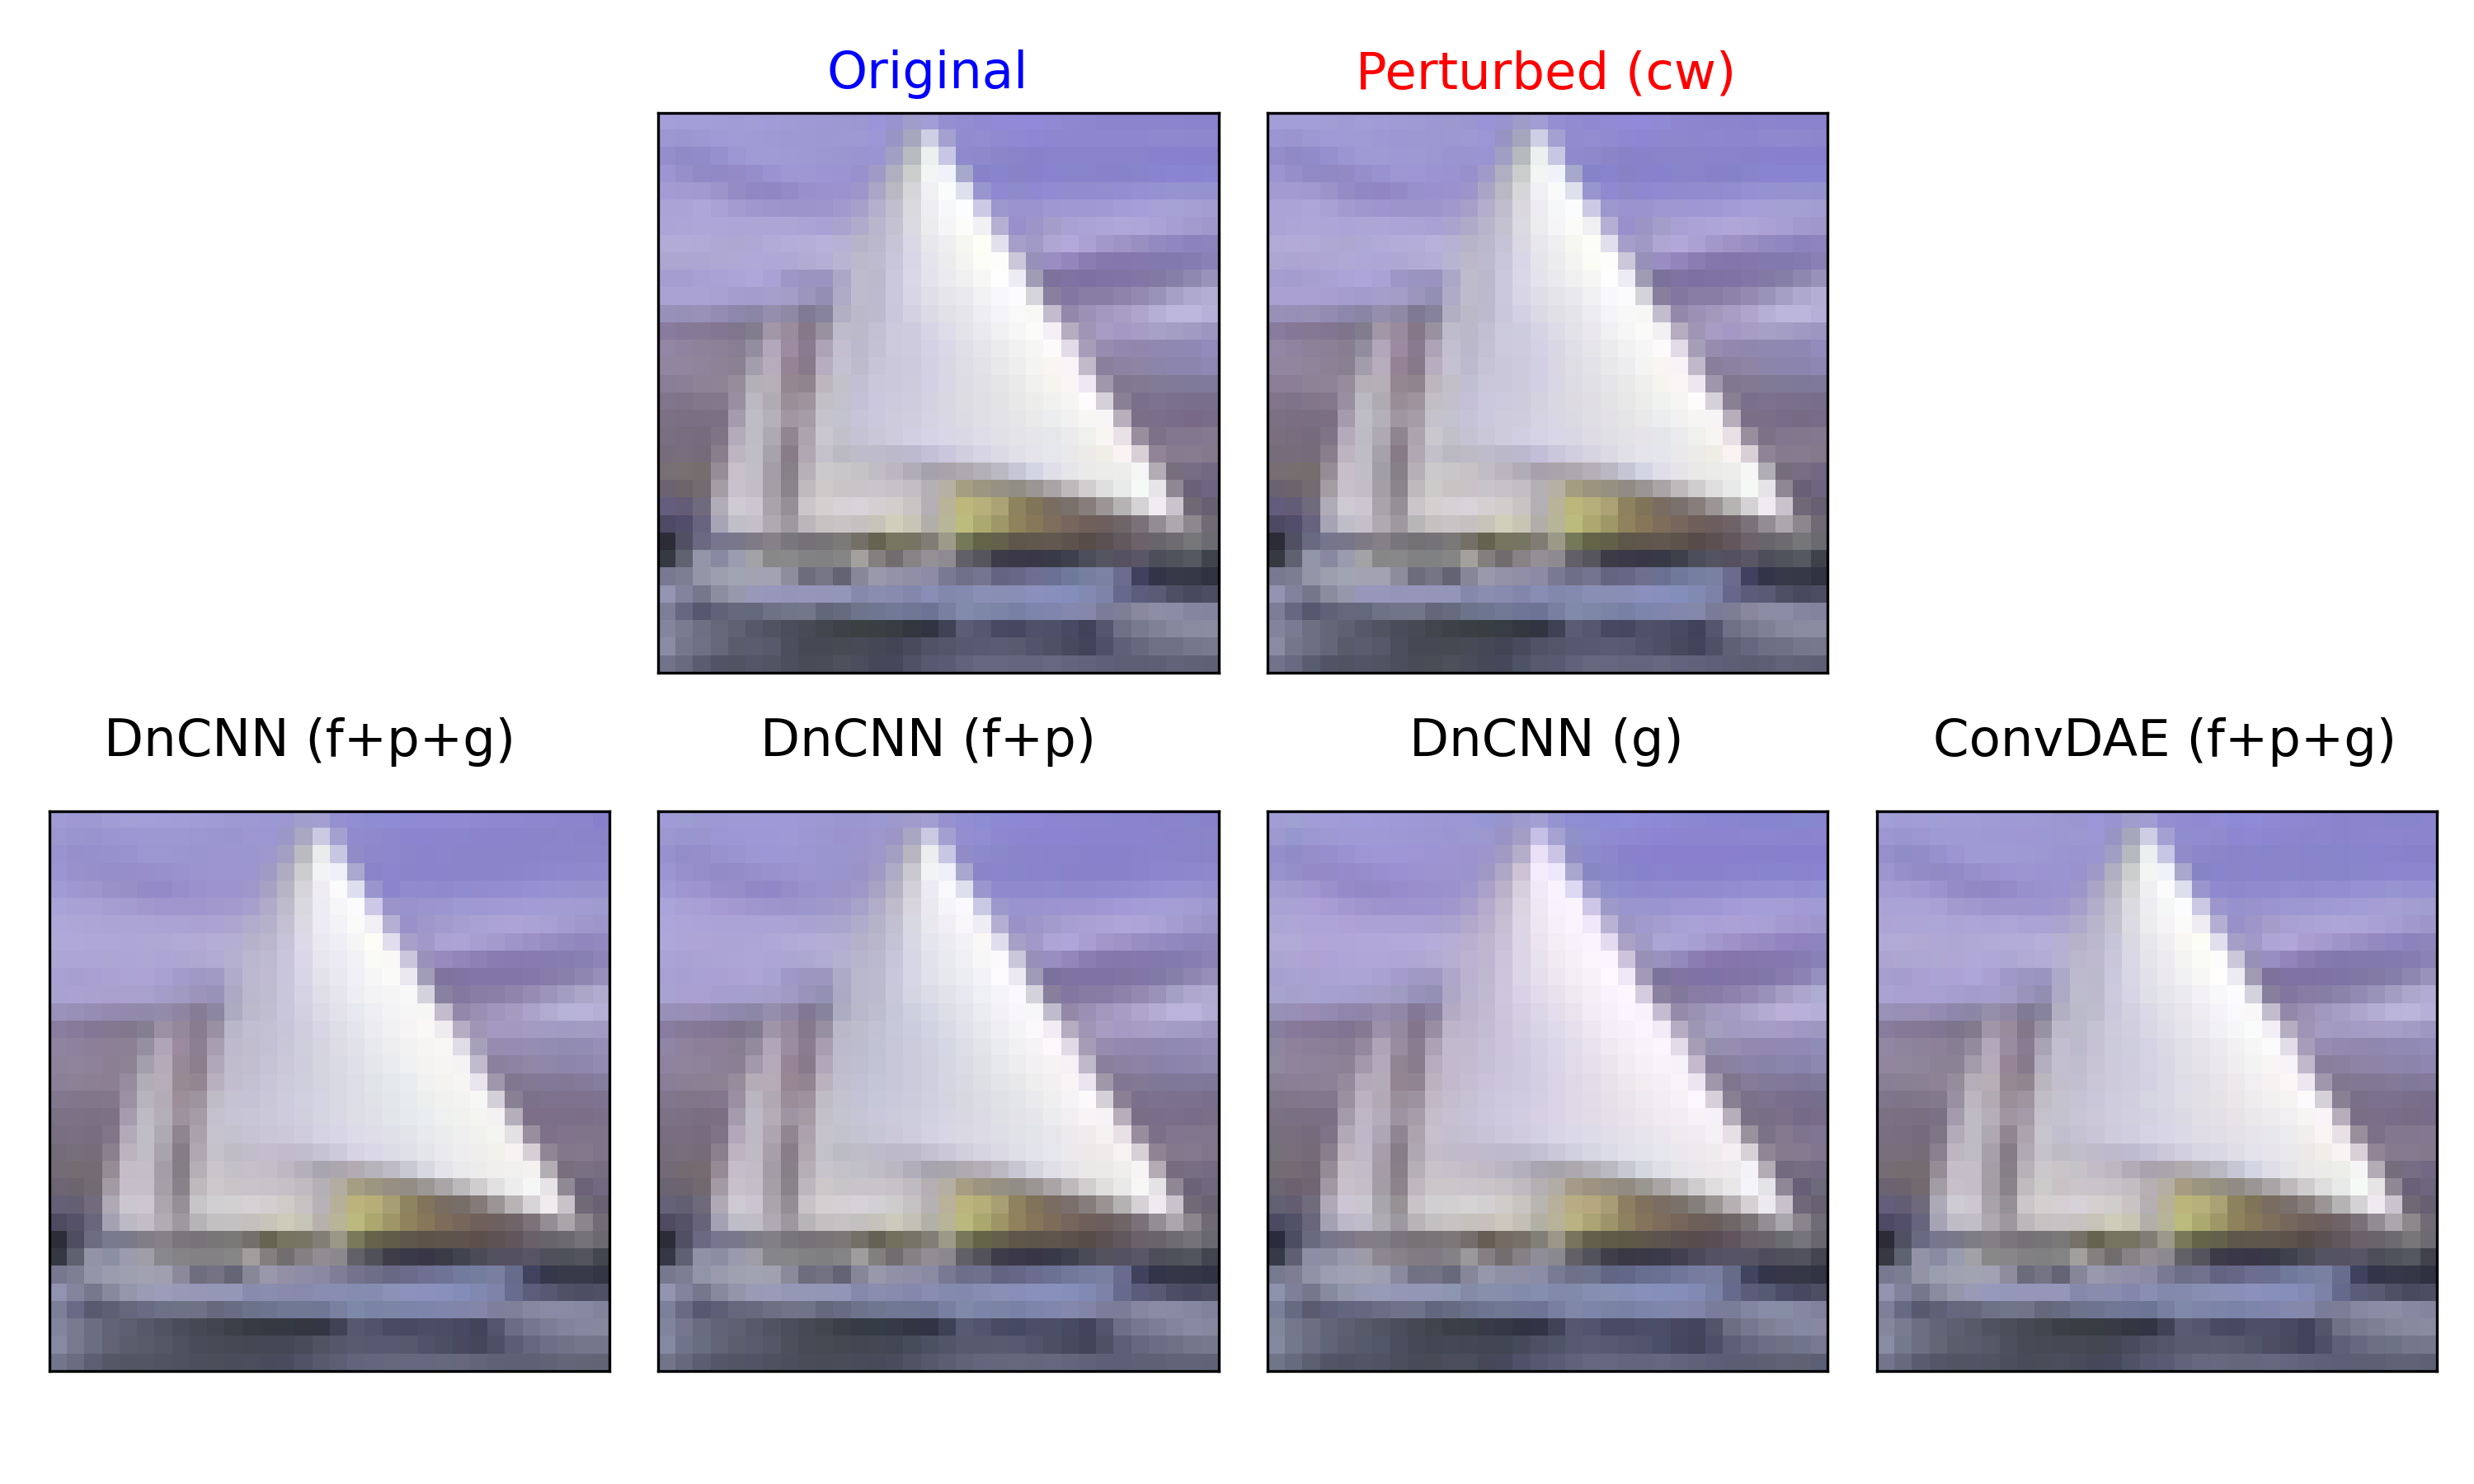
\includegraphics[width=\columnwidth]{images/cw_denoiser_comp2.png}
%     \caption{Sample C\&W image and denoiser outputs}
%     \label{fig:cw}
% \end{figure}



\subsection{Denoiser + Ensemble}

\begin{figure*}[!h]
\centering
    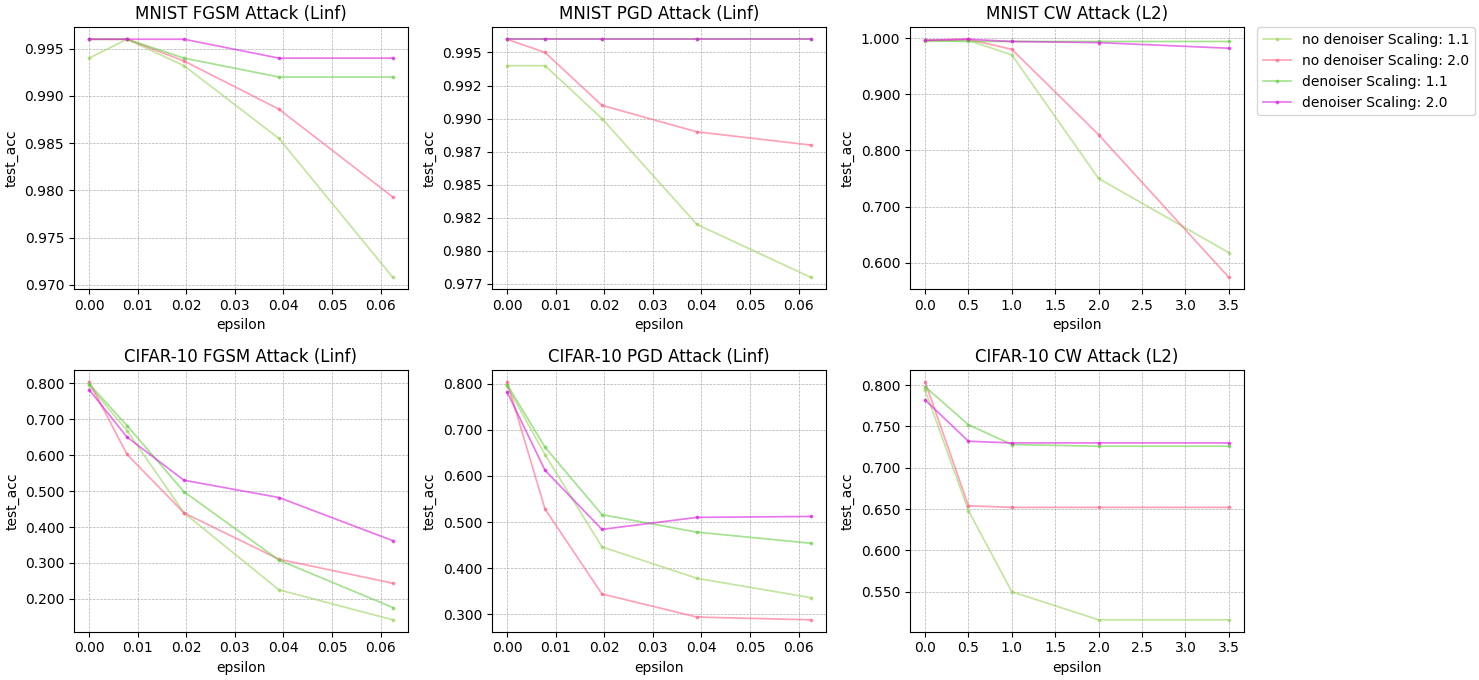
\includegraphics[scale=0.45]{images/denoiser_comparison.png}
    \caption{Effects of including a denoiser to the ensemble.}
    \label{fig:denoisercomp}
\end{figure*}
The combination of the denoiser and ensemble components produces significant improvements over simply the ensemble model, particularly at high perturbations and with stronger attacks (See Fig. \ref{fig:denoisercomp}). We note up to a 40.8\% and 21.0\% accuracy improvement in MNIST and CIFAR10, respectively, in the C\&W attack.

\begin{figure*}[!h]
\centering
    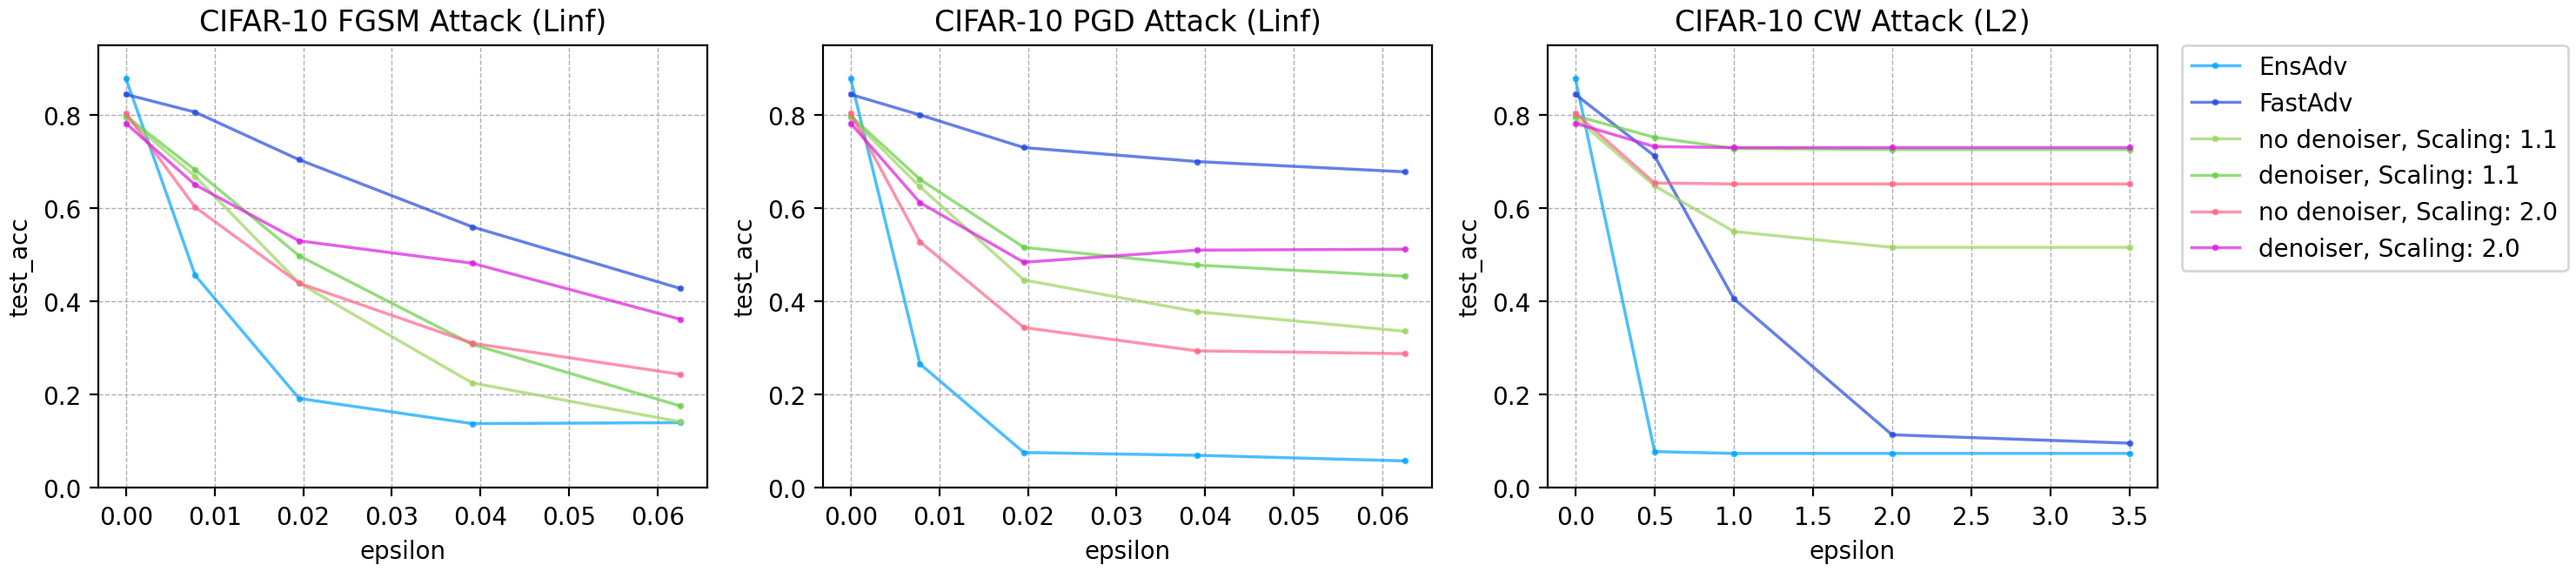
\includegraphics[scale=0.45]{images/comparison.png}
    \caption{Comparison with Ensemble Adversarial Training (EnsAdv) and Fast Adversarial Training (FastAdv).}
    \label{fig:comparison}
\end{figure*}
Lastly, in Fig. \ref{fig:comparison}, we compare the performance of our strongest ensemble models across both scaling factors against Ensemble Adversarial Training (EnsAdv) and Fast Adversarial Training (FastAdv). We can see that FastAdv, which improves upon EnsAdv, outperforms our method on both FGSM and PGD attacks. However, the combination of our denoiser and ensemble steps is able to outperform both FastAdv and EnsAdv by up to 63\% at the maximum perturbation level.


\section{Conclusion and Future Work} %%%%%%%%%%%%%%%%%%%%%%%%%%%%%%%%%%%
We have shown that the combination of the ensemble defense system and an adversarially trained denoising preprocessor provides a robust layer of protection against adversarial attacks. Our system was able to outperform the previously proposed ensemble-based defense system (Ensemble Adversarial Training) in all attacks tested, and edge over the Fast Adversarial Training method in the strongest tested C\&W attack.

Our system's capability can also be extended to more complex models and larger datasets, such as ImageNet. There is also the opportunity to explore non-differentiable up and down sampling methods for the image resizing step to add another layer of non-differentiability against potential attacks. Additionally, adversarial training could potentially be incorporated into the training we performed in each ensemble member. 


\bibliographystyle{IEEEtran}

% \bibliographystyle{plain}
%\bibliography{references}
\begin{thebibliography}{}
 \bibitem[1]{pbba} N. Papernot, P. McDaniel, I. Goodfellow, S. Jha, Z. B. Celik, and A. Swami, “Practical black-box attacks against machine learning,” in Proceedings of the 2017 ACM on Asia conference on computer and communications security, 2017, pp. 506-519.
 \bibitem[2]{fgsm} I. J. Goodfellow, J. Shlens, and C. Szegedy, “Explaining and harnessing adversarial examples,” arXiv preprint arXiv:1412.6572, 2014.
 \bibitem[3]{eat} F. Tramèr, A. Kurakin, N. Papernot, I. Goodfellow, D. Boneh, and P. McDaniel, “Ensemble adversarial training: Attacks and defenses,” arXiv preprint arXiv:1705.07204, 2017.
 \bibitem[4]{pgd} A. Madry, A. Makelov, L. Schmidt, D. Tsipras, and A. Vladu, “Towards deep learning models resistant to adversarial attacks,” arXiv preprint arXiv:1706.06083, 2017.
 \bibitem[5]{cw} N. Carlini and D. Wagner, “Towards evaluating the robustness of neural networks,” in 2017 ieee symposium on security and privacy (sp), 2017, pp. 39–57.
 \bibitem[6]{sgm} D. Wu, Y. Wang, S.-T. Xia, J. Bailey, and X. Ma, “Skip connections matter: On the transferability of adversarial examples generated with resnets,” arXiv preprint arXiv:2002.05990, 2020.
 \bibitem[7]{survey} F. Tramer, N. Carlini, W. Brendel, and A. Madry, “On adaptive attacks to adversarial example defenses,” Advances in Neural Information Processing Systems, vol. 33, pp. 1633–1645, 2020.
 \bibitem[8]{empir} S. Sen, B. Ravindran, and A. Raghunathan, “Empir: Ensembles of mixed precision deep networks for increased robustness against adversarial attacks,” arXiv preprint arXiv:2004.10162, 2020.
 \bibitem[9]{bpda} A. Athalye, N. Carlini, and D. Wagner, “Obfuscated gradients give a false sense of security: Circumventing defenses to adversarial examples,” in International conference on machine learning, 2018, pp. 274–283.
 \bibitem[10]{diversity} T. Pang, K. Xu, C. Du, N. Chen, and J. Zhu, “Improving adversarial robustness via promoting ensemble diversity,” in International Conference on Machine Learning, 2019, pp. 4970–4979.
 \bibitem[11]{cite11} Lee, S., Lee, J., and Park, S. (2018). Defensive denoising methods against adversarial attack. 
 \bibitem[12]{cite12} Maaten, L. V. D., Yuille, A. L., and He, K. (2019). Feature Denoising for Improving Adversarial Robustness. 2019 IEEE/CVF Conference on Computer Vision and Pattern Recognition (CVPR).
 \bibitem[13]{cite13} Bakhti, Y., Fezza, S. A., Hamidouche, W., and Deforges, O. (2019). DDSA: A Defense Against Adversarial Attacks Using Deep Denoising Sparse Autoencoder. IEEE Access, 7, 160397–160407.
 \bibitem[14]{cite14} Liao, F., Liang, M., Dong, Y., Pang, T., Hu, X., and Zhu, J. (2018). Defense Against Adversarial Attacks Using High-Level Representation Guided Denoiser. 2018 IEEE/CVF Conference on Computer Vision and Pattern Recognition.
 \bibitem[15]{cite15} Zuo, W., Chen, Y., Meng, D., and Zhang, L. (2017). Beyond a Gaussian Denoiser: Residual Learning of Deep CNN for Image Denoising. IEEE Transactions on Image Processing, 26(7), 3142–3155.
 \bibitem[16]{lbfgs} C. Szegedy et al., “Intriguing properties of neural networks,” arXiv preprint arXiv:1312.6199, 2013. 
 \bibitem[17]{dd} N. Papernot, P. McDaniel, X. Wu, S. Jha, and A. Swami, “Distillation as a defense to adversarial perturbations against deep neural networks,” in 2016 IEEE symposium on security and privacy (SP), 2016, pp. 582–597. 
 \bibitem[18]{fat}E. Wong, L. Rice, and J. Z. Kolter, “Fast is better than free: Revisiting adversarial training,” 2019. 
 \bibitem[19]{resnet} K. He, X. Zhang, S. Ren, and J. Sun, “Identity mappings in deep residual networks,” in European conference on computer vision, 2016, pp. 630–645.
 \bibitem[20]{rednet} X.-J. Mao, C. Shen, and Y.-B. Yang, “Image Restoration Using Convolutional Auto-encoders with Symmetric Skip Connections,” CoRR, vol. abs/1606.08921, 2016

\end{thebibliography}



\end{document}


